% \chapter{Feature extraction}
\chapter{特征提取}
\label{chap:feature_extraction}

% A robot can obtain information about its environment by both active (e.g., ultra-sound, light, and laser) or passive sensing (e.g., acceleration, magnetic field, or cameras). There are only few cases where this information is directly useful to a robot. Before being able to arrive at semantic information such as ``I'm in the kitchen'', ``this is a cup'' or ``this is a horse'', is identifying higher-level \emph{features}.\index{Features}

% The goal of this chapter is to introduce a series of standard feature detectors such as the

机器人可以通过主动感知(例如超声、光和激光)或被动感知(例如加速度、磁场或照相机)获得关于环境的信息。但是只有少数情况下,这些信息对机器人直接有用。在能够得到诸如“我在厨房”、“这是一个杯子”或者“这是一匹马”之类的语义信息之前,机器人需要能够识别高级\emph{特征(Features)}\index{特征(Features)}。

本章的目标是引入一系列标准的特征检测器,如

\begin{itemize}
% \item Hough-transform to detect lines, circles and other shapes,
% \item numerical methods such as least-squares, split-and-merge and RANSAC to find high-level features in noisy data,
% \item Scale-invariant features.

\item 霍夫变换可以检测直线、圆和其他形状
\item 在噪声数据中找到高级特征的数值方法,如最小二乘法、分割合并和RANSAC
\item 缩放不变的特征
\end{itemize}

% \section{Feature detection as an information-reduction problem}
% The information generated by sensors can be quite formidable. For example, a simple webcam generates 640x480 color pixels (red, green and blue) or 921600 Bytes around 30 times per second. A single-ray laser scanner still provides around 600 distance measurements 10 times per second. This is in contrast to the information that a robot actually requires. Consider for example the maze-solving competition ``Ratslife'' (Section \ref{sec:ratslife}) in which the robot's camera can be used to recognize one of 48 different color patterns (Figure \ref{fig:ratslife}) that are distributed in the environment, or the presence or absence of a charger, essentially reducing hundreds of bytes of camera data to around 6 bit ($2^6=64$ different values) content. The goal of most image processing algorithms is therefore to first reduce information content in a meaningful way and then extract relevant information. In chapter \ref{chap:vision}, we have seen convolution-based filters such as blurring, detecting edges, or binary operations such as thresholding. We are now interested in methods to extract higher-level features such as lines and techniques to extract them.

\section{把特征检测看作信息减少问题}

传感器产生的信息数量惊人。例如,简单的网络摄像头大约每秒生成30次$640\times 480$个彩色像素(红色,绿色和蓝色)或921600字节。单射线激光扫描仪可提供约每秒10次,每次600个测距值。这与机器人实际需要的信息相反。例如,考虑迷宫求解比赛“Ratslife”(第\ref{sec:ratslife}节),其中机器人的相机可识别48种分布在环境中不同的颜色图案的一种(图\ref{fig:ratlife}),或检测充电桩存不存在,基本上将数百字节的摄像机数据减少到大约6位($2^6=64$不同值)。因此,大多数图像处理算法的目标是首先以有意义的方式减少信息内容,然后提取相关信息。在第\ref{chap:vision}章中,我们已经讲了基于卷积的过滤器,例如模糊、边缘检测或二进制操作(如阈值)。现在我们对提取高级特征(如直线),以及提取它们的方法感兴趣。


% \section{Features}
\section{特征}

% Lines are particularly useful features for localization and can correspond to walls in laser scans, markers on the floor or corners detected in a camera image. Whereas a Sobel filter (Section \ref{sec:sobel}) can help us to highlight lines and edges in images, additional algorithms are needed to extract structured information such as the orientation and position of a line with respect to the robot.

直线是特别有用的定位特征,可以对应激光扫描中的墙壁、地面上的标记或摄像机图像中检测到的角落。虽然Sobel过滤器(第\ref{sec:sobel}节)可以帮助我们突出图像中的直线和边缘,但是我们需要额外的算法来提取结构化信息,例如直线相对于机器人的方向和位置。

% A desirable property of a feature is that its extraction is repeatable and robust to rotation, scale, and noise in the data. We need feature detectors that can extract the same feature from sensor data, even if the robot has slightly turned or moved farther or closer to the feature. There are many feature detectors available that accomplish this, prominent examples are the Harris corner detector\index{Harris Corner Detector} (essentially detecting points in the image where vertical and horizontal lines cross) and the SIFT feature detector\index{SIFT features}. Feature detection is important far beyond robotics and is for example used in hand-held cameras that can automatically stitch images together. Here, feature detectors will ``fire'' on the same features in two images taken from slightly different perspectives, which allows the camera to calculate the transformation between the two.

我们期望提取的特征对旋转、缩放和数据中的噪声是可重复的和鲁棒的。我们需要能够从传感器数据中提取相同特征的特征检测器,即使机器人稍微转动或移动得离这个特征更远或更近。有许多特征检测器可以实现这一点,著名的例子有Harris拐角检测器(Harris Corner Detector)\index{Harris拐角检测器(Harris Corner Detector)}(基本上是检测图像中垂直和水平线的交叉点)和SIFT特征检测器\index{SIFT特征}。特征检测在机器人领域之外也是非常重要的,例如用在可以自动将图像拼接在一起的手持相机中。在这里,从稍微不同的角度拍摄的两个图像中的相同特征上特征检测器会“触发”,这使得相机可以计算两个图像之间的转换。

% This chapter focuses on two important classes of features: line features and scale-invariant features in images (SIFT). Both features provide tangible example for the least-squares and RANSAC algorithms, which are also introduced in this chapter. Both features are representative for a large class of detectors, and have been chosen for their simplicity, providing a basis for understanding the function of more complex feature detectors.

本章重点介绍两个重要的特征:图像中的直线特征和尺度不变特征(SIFT)。这两个特征为最小二乘法和RANSAC算法提供了实际的例子,本章也将介绍这一点。这两个特征是一大类检测器的代表,因为简单而被选择,它们为理解更复杂的特征检测器提供了基础。


% \section{Line recognition}
\section{直线识别}

% Why are lines a useful feature? As you will see next chapter, the key challenge in estimating a robot's pose is unreliable odometry, in particular when it comes to turning. Here, a simple infrared sensor measuring the distance to a wall can provide the robot with a much better feel for what actually happened. Similarly, if a robot has the ability to track markers in the environment using vision, it gets another estimate on how much it is actually moving. How information from odometry and other sensors can be fused not only to localize the robot, but also to create maps of its environment, will be the focus of the remainder of this book.

为什么直线是有用的特征?正如下一章你将看到的,机器人姿势估计的关键挑战是不可靠的测距,特别是转弯时。这里,测量与墙壁距离的简单红外传感器可以为机器人提供更好的对环境的认知。类似地,如果机器人能够使用视觉跟踪环境中的标记,则可以对其实际移动大小进行额外估计。如何将测距仪和其他传感器的信息融合在一起,不仅可以使机器人定位,还可以创建其环境的地图,这将是本书剩余章节的重点。

% A laser scanner or similar device pointed against a wall will return a suite of $N$ points at position $(x_i,y_i)$ in the robot's coordinate system. These points can also be represented in polar coordinates $ (\rho_i,\theta_i)$. We can now imagine a line running through these points that is parametrized with a distance $r$ and an angle $\alpha$. Here, $r$ is the distance of the robot to the wall and $ \alpha$ its angle. As all sensors are noisy, each point will have distance $d_i$ from the ``optimal'' line running through the points. These relationships are illustrated in Figure \ref{fig:linefitting}.

指向墙壁的激光扫描仪或类似装置将在机器人坐标系中的位置$(x_i,y_i)$处返回$N$个点。这些点也可以用极坐标$(\rho_i,\theta_i)$表示。我们现在可以想象一条线穿过这些以距离$r$和角度$\alpha$参数化的点。这里,$r$是机器人与墙壁的距离,$\alpha$是它的角度。由于所有传感器都有噪声,所以每个点距离“最优”直线的距离为$d_i$。这些关系如图\ref{fig:linefitting}所示。

\begin{figure}
	\centering
		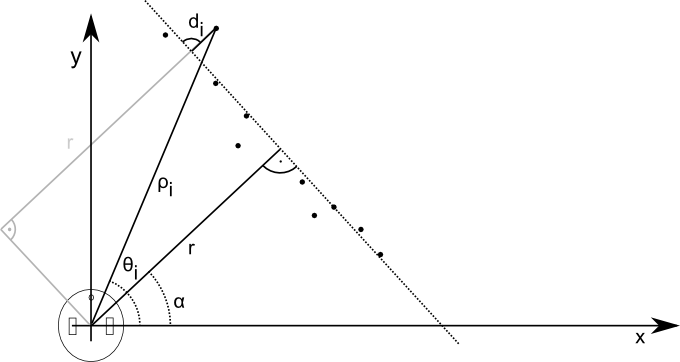
\includegraphics[width=\textwidth]{figs/linefitting.png}
	% \caption{A 2D point cloud recorded by a laser-scanner or similar device. A line (dashed) is fitted through the points in a least-square sense.}
	\caption{由激光扫描仪或类似装置记录的2D点云。直线(虚线)以最小二乘的方式穿过这些点。}
	\label{fig:linefitting}
\end{figure}

% \subsection{Line fitting using least squares}
\subsection{使用最小二乘法的直线拟合}
% Using simple trigonometry we can now write

使用简单的三角学我们现在可以写为

\begin{equation}
\rho_i \cos(\theta_i-\alpha)-r=d_i.
\end{equation}

% Different line candidates --- parametrized by $ r$ and $ \alpha$ --- will have different values for $ d_i$. We can now write an expression for the total error $ S_{r,\alpha}$ as

由$r$和$\alpha$进行参数化的不同候选直线对于$d_i$有不同的值。现在我们可以将总误差$S_{r,\alpha}$表示为


\begin{equation}
S_{r,\alpha}=\sum_{i=1}^{N}{d_i^2}=\sum_i(\rho_i \cos(\theta_i-\alpha)-r)^2
\end{equation}

% Here, we square each individual error to account for the fact that a negative error, i.e.\a point left of the line, is as bad as a positive error, i.e.\a point right of the optimal line. In order to optimize $ S_{r,\alpha}$, we need to take the partial derivatives with respect to $ r$ and $ \alpha$, set them zero, and solve the resulting system of equations for $ r$ and $ \alpha$.

在这里,我们将每个单独的误差看作:一个负误差为该直线左边的一个点,一个正误差为该直线右边的一个点。为了优化$S_{r,\alpha}$,我们需要对$r$和$\alpha$取偏导数,然后令它们为零求解关于$r$和$\alpha$的方程组。

\begin{equation}
\frac{\partial{S}}{\partial{\alpha}}=0 \qquad \frac{\partial{S}}{\partial{r}}=0
\end{equation}

% Here, the symbol $ \partial$ indicates that we are taking a partial derivative. Solving for $r$ and $\alpha$ is involved, but possible \cite{siegwart2011introduction}:

这里,符号$\partial$表示取偏导数。求解$r$和$\alpha$是复杂但可能的\cite{siegwart2011introduction}:

\begin{equation}\label{eq:linealpha}
\alpha=\frac{1}{2}atan\left(\frac{\frac{1}{N}\sum{\rho_i^2 sin 2\theta_i}-\frac{2}{N^2}\sum{\sum{\rho_i\rho_j cos \theta_i sin \theta_j}}}{\frac{1}{N}\sum{\rho_i^2 cos 2 \theta_i - \frac{1}{N^2}\sum{\sum{\rho_i \rho_j cos(\theta_i+\theta_j)}}}}\right)
\end{equation}

% and
和

\begin{equation}\label{eq:liner}
r=\frac{{\sum \rho_i cos (\theta_i-\alpha)}}{N}
\end{equation}

% We can therefore calculate the distance and orientation of a wall captured by our proximity sensors relative to the robot's positions or the height and orientation of a line in an image based on a collection of points that we believe might belong to a line.

因此,我们可以计算由距离传感器获得的墙壁相对于机器人的距离和方向,或基于我们认为属于同一直线的点集合计算图像中直线的高度和方向。

% This approach is known as the \emph{least-square method}\index{Least-Square Method (Line fitting)} and can be used to fit data to any parametric model. The general approach is to describe the fit between the data and the model in terms of an error. The best fit will minimize this function, which will therefore have a zero derivative at this point. If the result cannot be obtained analytically as in this example, numerical methods have to be used to find the best fit that minimizes the quadratic error.

这种方法称为\emph{最小二乘法(Least-Square Method)}\index{最小二乘法(Least-Square Method)(直线拟合,Line fitting))},可用于将数据拟合到任何参数模型中。一般的方法是利用误差来描述数据和模型之间的拟合。最佳拟合将最小化这个方程,因此在这一点上会有一个零导数。如果在这个例子中不能解析地求得结果,则必须使用数值方法来找出最小化这个二次误差的最佳拟合。

% \subsection{Split-and-merge algorithm}
% A key problem with this approach is that it is often unclear how many lines there are and where a line starts and where it ends. Looking through the camera, for example, we will see vertical lines corresponding to wall corners and horizontal ones that correspond to wall-floor intersections and the horizon; using a distance sensor, the robot might detect a corner. We therefore need an algorithm that can separate point clouds into multiple lines. One possible approach is to find the outlier with the strongest deviation from a fitted line and split the line at this point. This is illustrated in Figure \ref{fig:splitandmerge}. This can be done iteratively until each line has no outliers above a certain threshold.

\subsection{分割合并算法}

这种方法的一个关键问题是,我们通常不清楚有多少条直线,以及每条直线起始以及结束的位置。例如,通过相机我们看到对应于墙壁拐角的垂直线和对应于墙-地和地平线的水平线;使用距离传感器,机器人可能会检测到拐角。因此,我们需要一种可将点云分成多条直线的算法。一种可能的方法是找出与拟合线偏离最大的异常值,并以此点分割。这在图\ref{fig:splitandmerge}中说明。这可以迭代地进行,直到每一条直线都没有高于某个阈值的异常值。


\begin{figure}
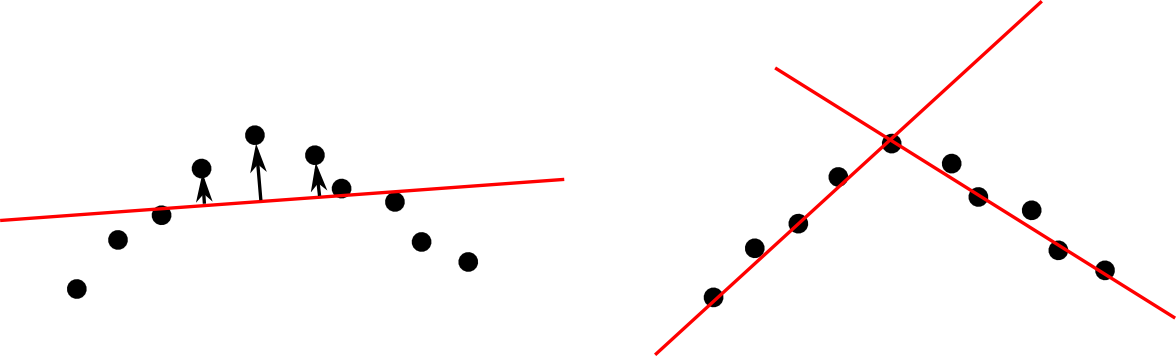
\includegraphics[width=\textwidth]{figs/splitandmerge}
% \caption{Split-and-merge algorithm. Initial least-square fit of a line (left). Splitting the data-set at the point with the highest error (after picking a direction) allows fitting two lines with overall lesser error.\label{fig:splitandmerge}}
\caption{
分割合并算法。直线的初始最小二乘拟合(左)。(选择方向之后)在误差最高的点上分割数据集可以拟合两条总体误差较小的直线。
\label{fig:splitandmerge}}
\end{figure}

% \subsection{RANSAC: Random Sample and Consensus}
% If the number of ``outliers'' are large, a least square fit will generate poor results as it will generate the ``best'' fit that accomodates both ``inliers'' and ``outliers''. Also, split-and-merge algorithms will fail as they are extremely susceptive to noise: depending on the actual parameters every outlier will split a potential line into two. A solution to this problem is to randomly sample possible lines and keep those that satisfy a certain desired quality given by the number of points being somewhat close to the best fit. This is illustrated in Figure \ref{fig:ransac}, with darker lines corresponding to better fits. RANSAC\index{RANSAC}\index{Random Sample and Consensus} usually requires two parameters, namely the number of points required to consider a line to be a valid fit, and the maximum $d_i$ from a line to consider a point an inlier and not an outlier. The algorithm proceeds as follows: select two random points from the set and connect them with a line. Grow this line by $d_i$ in both directions and count the number of inliers. Repeat this until one or more lines that have sufficient number of inliers are found, or a maximum number of iterations are reached.

\subsection{随机抽样与共识(Random Sample and Consensus,RANSAC)}

如果“异常值”的数量很大,那么最小二乘拟合会产生很差的结果,因为它会产生同时适应“正常值”和“异常值”的“最佳”拟合。此外,分割合并算法将会失败,因为它们对噪声非常敏感:根据实际参数,每个异常值都将可能的直线分成两部分。这个问题的解决方案是随机抽取可能的直线,并基于靠近最佳拟合点的数目,保留那些达到一定期望质量的直线。这在图\ref{fig:ransac}中示出,其中较黑的直线对应于更好的拟合。RANSAC\index{随机抽样与共识(Random Sample and Consensus,RANSAC)}通常需要两个参数,即判定直线为有效拟合所需点的数目,以及判定正常点或异常点的最大$d_i$。算法执行如下:从集合中选择两个随机点,并将它们相连。将直线在两个方向上各增加$d_i$,计算正常点的数量。重复此操作,直到找到具有足够数量正常点的一条或多条直线,或者达到最大迭代次数。

\begin{figure}
\center
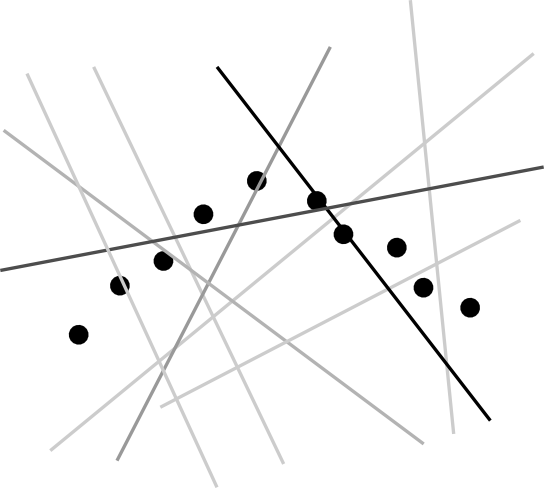
\includegraphics[width=0.6\textwidth]{figs/ransac}
% \caption{Random Sample and Consensus (RANSAC). Random lines are evaluated by counting the number of points close by (''inliers''), darker lines are better fits.\label{fig:ransac}}
\caption{
RANSAC。通过计数邻近点(“正常点”)的数量来评估随机直线,较黑的直线表示拟合更好。
\label{fig:ransac}}
\end{figure}

% The RANSAC algorithm is fairly easy to understand in the line fitting application, but can be used to fit arbitrary parametric models to any-dimensional data. Here, its main strength is to cope with noisy data.

% Given that RANSAC is random, finding a really good fit will take quite some time. Therefore, RANSAC is usually used only as a first step to get an initial estimate, which can then be improved by some kind of local optimization, such as least-squares, e.g.

RANSAC算法在直线拟合应用中非常好理解,它还可以用于将任意参数模型拟合到任意维数据。在这里,它的主要优点是应对有噪声的数据。

鉴于RANSAC是随机的,找到一个非常好的拟合将需要相当长的时间。因此,RANSAC通常仅于获得初始估计,然后通过局部优化算法来改进,例如最小二乘法。


% \subsection{The Hough Transform}
% The Hough transform \index{Hough transform} can best be understood as a voting scheme to guess the parametrization of a feature such as a line, circle or other curve \cite{duda1972use}. For example, a line might be represented by $y=mx+c$, where $m$ and $c$ are the gradient and offset. A point in this parameter space (or ``Hough-space'') then corresponds to a specific line in $x-y$-space (or ``image-space''). The Hough-transform now proceeds as follows: for every pixel in the image that could be part of a line, e.g., white pixels in a thresholded image after Sobel filtering, construct all possible lines that intersect this point. (Drawing an image of this would look like a star). Each of these lines has a specifc $m$ and $c$ associated with it, for which we can add a white dot in Hough-space. Continuing to do this for every pixel of a line in an image will yield many $m-c$ pair, but only one that is common among all those pixels of the line in the image: the actual $m-c$ parameters of this line. Thinking about the number of times a point was highlighted in Hough-space as brightness, will turn a line in image space into a bright spot in Hough-space (and the other way round). In practice, a polar representation is chosen for lines. This is shown in Figure \ref{fig:hough}. The Hough transform also generalizes to other parametrization such as circles.

\subsection{霍夫变换}
可以把霍夫变换(Hough Transform)\index{霍夫变换(Hough Transform)}理解成一个投票方案来猜测诸如直线、圆或其他曲线特征的参数化\cite{duda1972use}。例如,一条直线可以由$y=mx+c$表示,其中$m$和$c$是斜率和截距。此参数空间(或“霍夫空间(Hough-space”)中的一个点对应于$x-y$空间(或“图像空间”)中的某条线。霍夫变换执行如下:对于可能是直线的一部分的图像中的每个像素(例如Sobel滤波之后的阈值图像中的白色像素),构造与该点相交的所有可能的直线。(绘制一个这样的图像看起来像一颗星星。)每一条直线都关联一对特定的$m$和$c$,我们可以在霍夫空间中为其添加一个白点。继续为图像中的的每条直线上的每个像素执行此操作,这会产生许多$m-c$对,但在图像的一条直线的所有像素中只有一对是一样的,即该直线的真实$m-c$参数。想象把点在霍夫空间突出的次数作为亮度,这会将图像空间中的一条线变成霍夫空间的亮点(反之亦然)。在实践中,我们把直线表示成极坐标。这显示在图\ref{fig:hough}中。霍夫变换也可以泛化为其他特征参数化,如圆。


\begin{figure}
\center
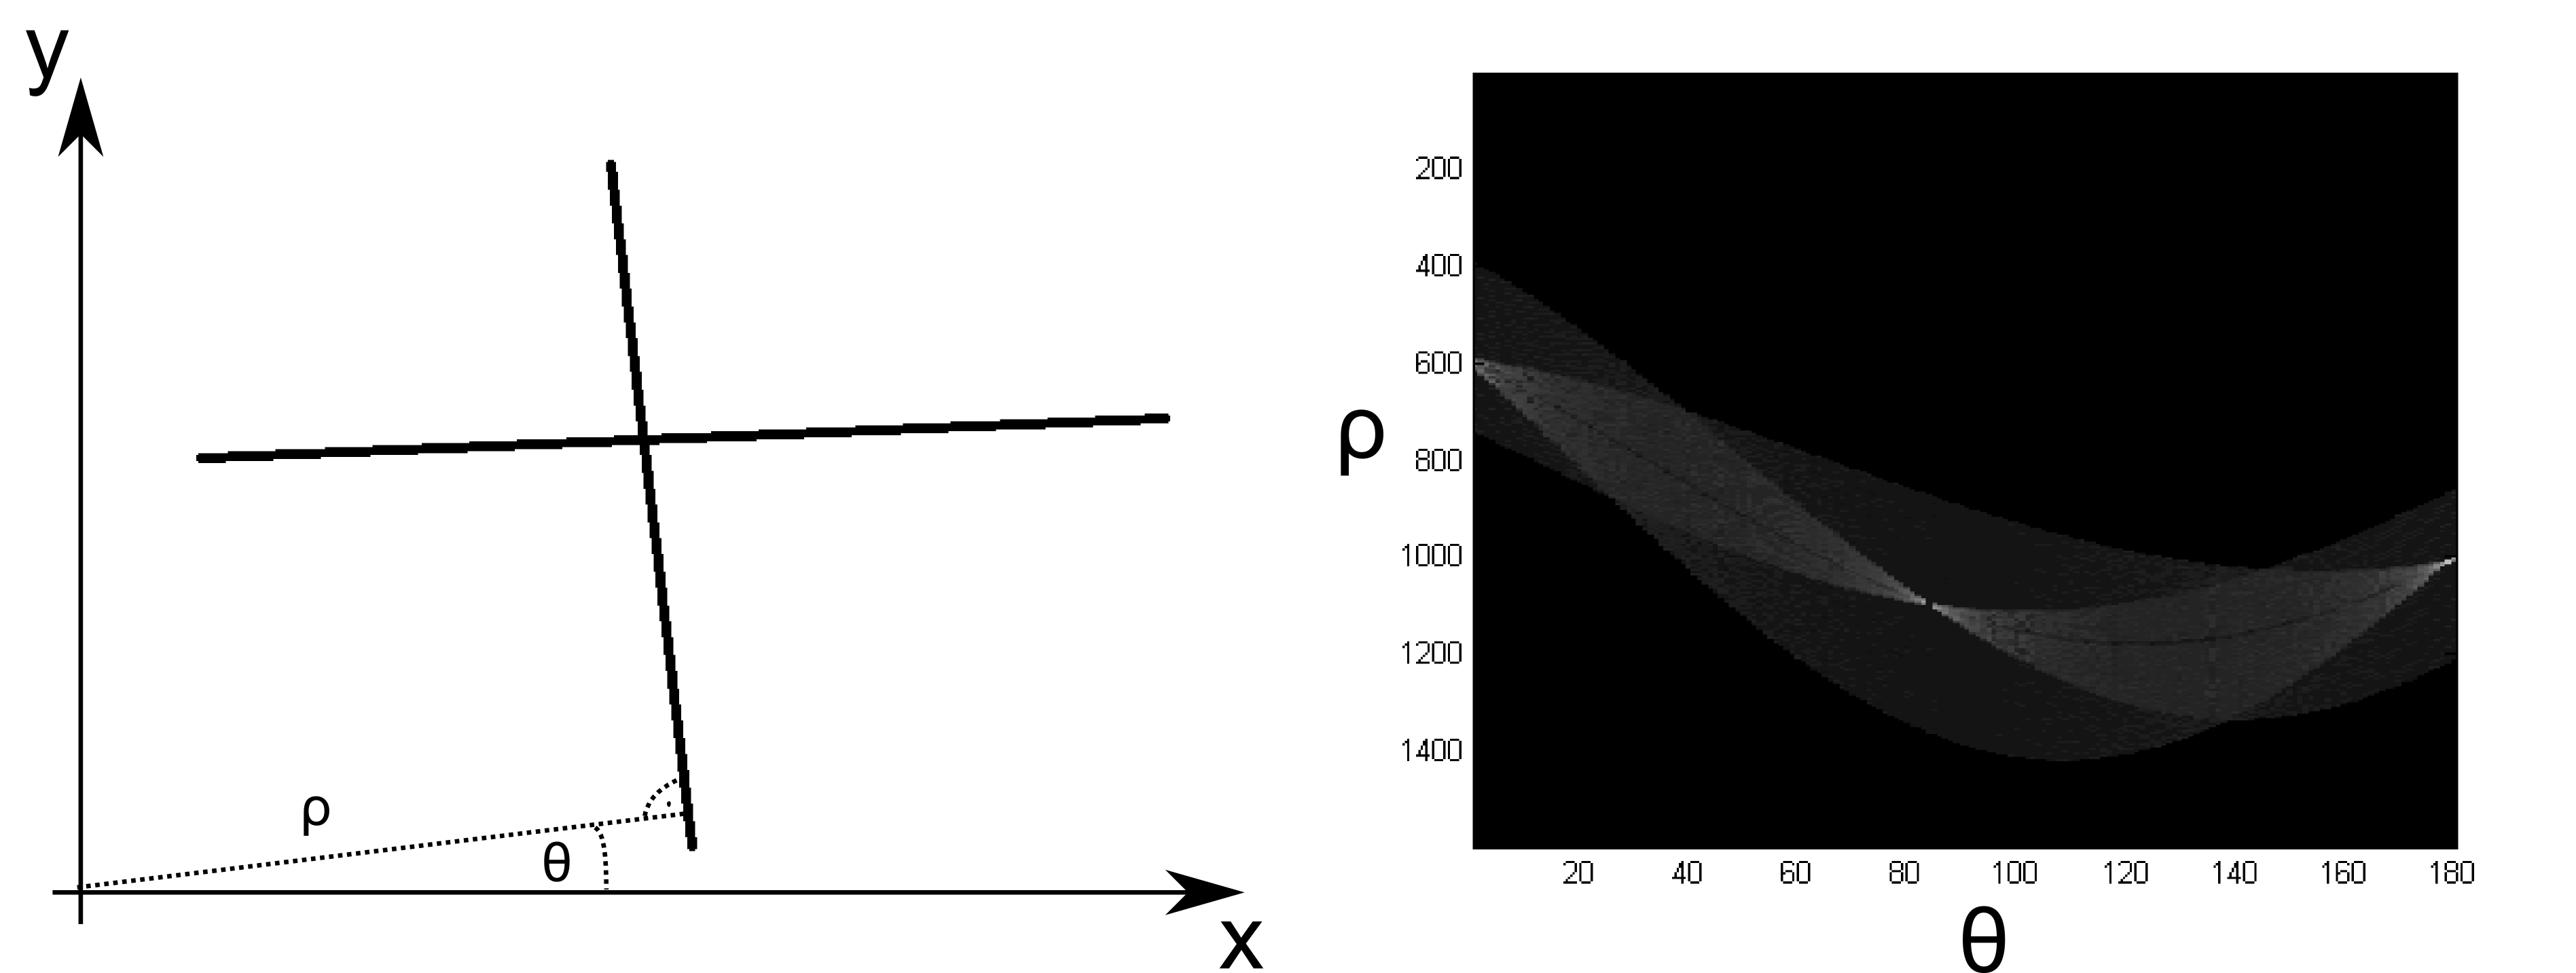
\includegraphics[width=\textwidth]{figs/houghtransform}
% \caption{Lines in an image (left) transposed into Hough-space $\rho$ (distance from origin) and $\theta$ (angle of normal with respect to origin). Bright spots in the Hough image (right) correspond to parameters that have received the most ``votes'' and clearly show the two lines at around 90$^o$ and 180$^o$.\label{fig:hough}}
\caption{
图像中的直线(左)转换到霍夫空间$\rho$(距原点的距离)和$\theta$(法线相对于原点的角度)。霍夫图像(右)中的亮点对应于获得最多“投票”的参数,并且清楚地显示了处于大约$90^o$和$180^o$的两条直线。
\label{fig:hough}}
\end{figure}


% \section{Scale-Invariant Feature Transforms}
% Scale-invariant feature transforms are a class of algorithms/signal-processing techniques that allow to extract features that are easily detectable across different scales (or distances to an object), independent of their rotation, and to some extent robust to affine transformations, i.e., views of the same object from different perspectives, and illumination changes. The most prominent in this class is the SIFT algorithm \cite{lowe1999object},\index{SIFT} which however has lost popularity due to closed-source and licensing cost, and has been replaced in the past with SURF (Speed-Up Robust Feature)\index{SURF} and many others,  which are freely available and have slightly different performance and varying use cases. As the math behind SURF is more involved, we focus on the intuition behind SIFT and encourage the reader to download and play with the various open-source implementations of other feature detectors that are available open source.

\section{尺度不变特征变换}

尺度不变特征变换是一类算法/信号处理技术,其允许提取在不同尺度(或离物体的距离)下容易检测的特征,独立与旋转,并且对仿射变换有某种程度的鲁棒性,即,从不同角度以及照明变化下同一个物体的影像。该类中最著名的是SIFT算法\cite{lowe1999object}\index{SIFT},然而由于闭源和许可成本,该算法已经不流行,并且已经被SURF(加速鲁棒特征(Speed-Up Robust Feature))\index{加速鲁棒特征(Speed-Up Robust Feature,SURF)}等其它算法取代,这些都是免费可得的,有稍微不同的性能和不同用途的用例。由于SURF背后更多地涉及数学,因此我们专注于SIFT背后的直观理解,我们也鼓励读者下载并使用其他开源的特征检测器的各种开源代码实现。


% \subsection{Overview}
% SIFT proceeds in multiple steps. Descriptions of the algorithm often include its application to object recognition, but these algorithms are independent of feature generation (see below).

\subsection{概述}

SIFT执行多个步骤。该算法的描述通常包括其物体识别的应用,但这些算法与特征生成无关(见下文)。

\begin{enumerate}
% \item Differences of Gaussians (DoG) at different scales:
\item 不同尺度的高斯差值(Differences of Gaussians,DoG):

\begin{itemize}
% \item Generate multiple scaled versions of the same image by re-sampling every 2nd, 4th and so on pixel.
% \item Filtering each scaled picture with various Gaussian filters of different variance.
% \item Calculating the difference between pairs of filtered images. This is equivalent to a DoG filter.

\item 对每隔2个像素、4个像素等进行重新采样,生成同一图像的多个缩放版本。
\item 使用不同方差的各种高斯滤波器过滤每个缩放图像。
\item 计算过滤图像对之间的差异。这相当于DoG过滤器。
\end{itemize}

% \item Detecting local minima and maxima in the DoG images across different scales (Figure \ref{fig:siftrejection}, left) and reject those with low contrast (Figure \ref{fig:siftrejection}, right).

\item 检测不同尺度的DoG图像中的局部最小值和最大值(图\ref{fig:siftrejection},左),并排除那些对比度低的图像(图\ref{fig:siftrejection},右)。

\begin{figure}
	\centering
		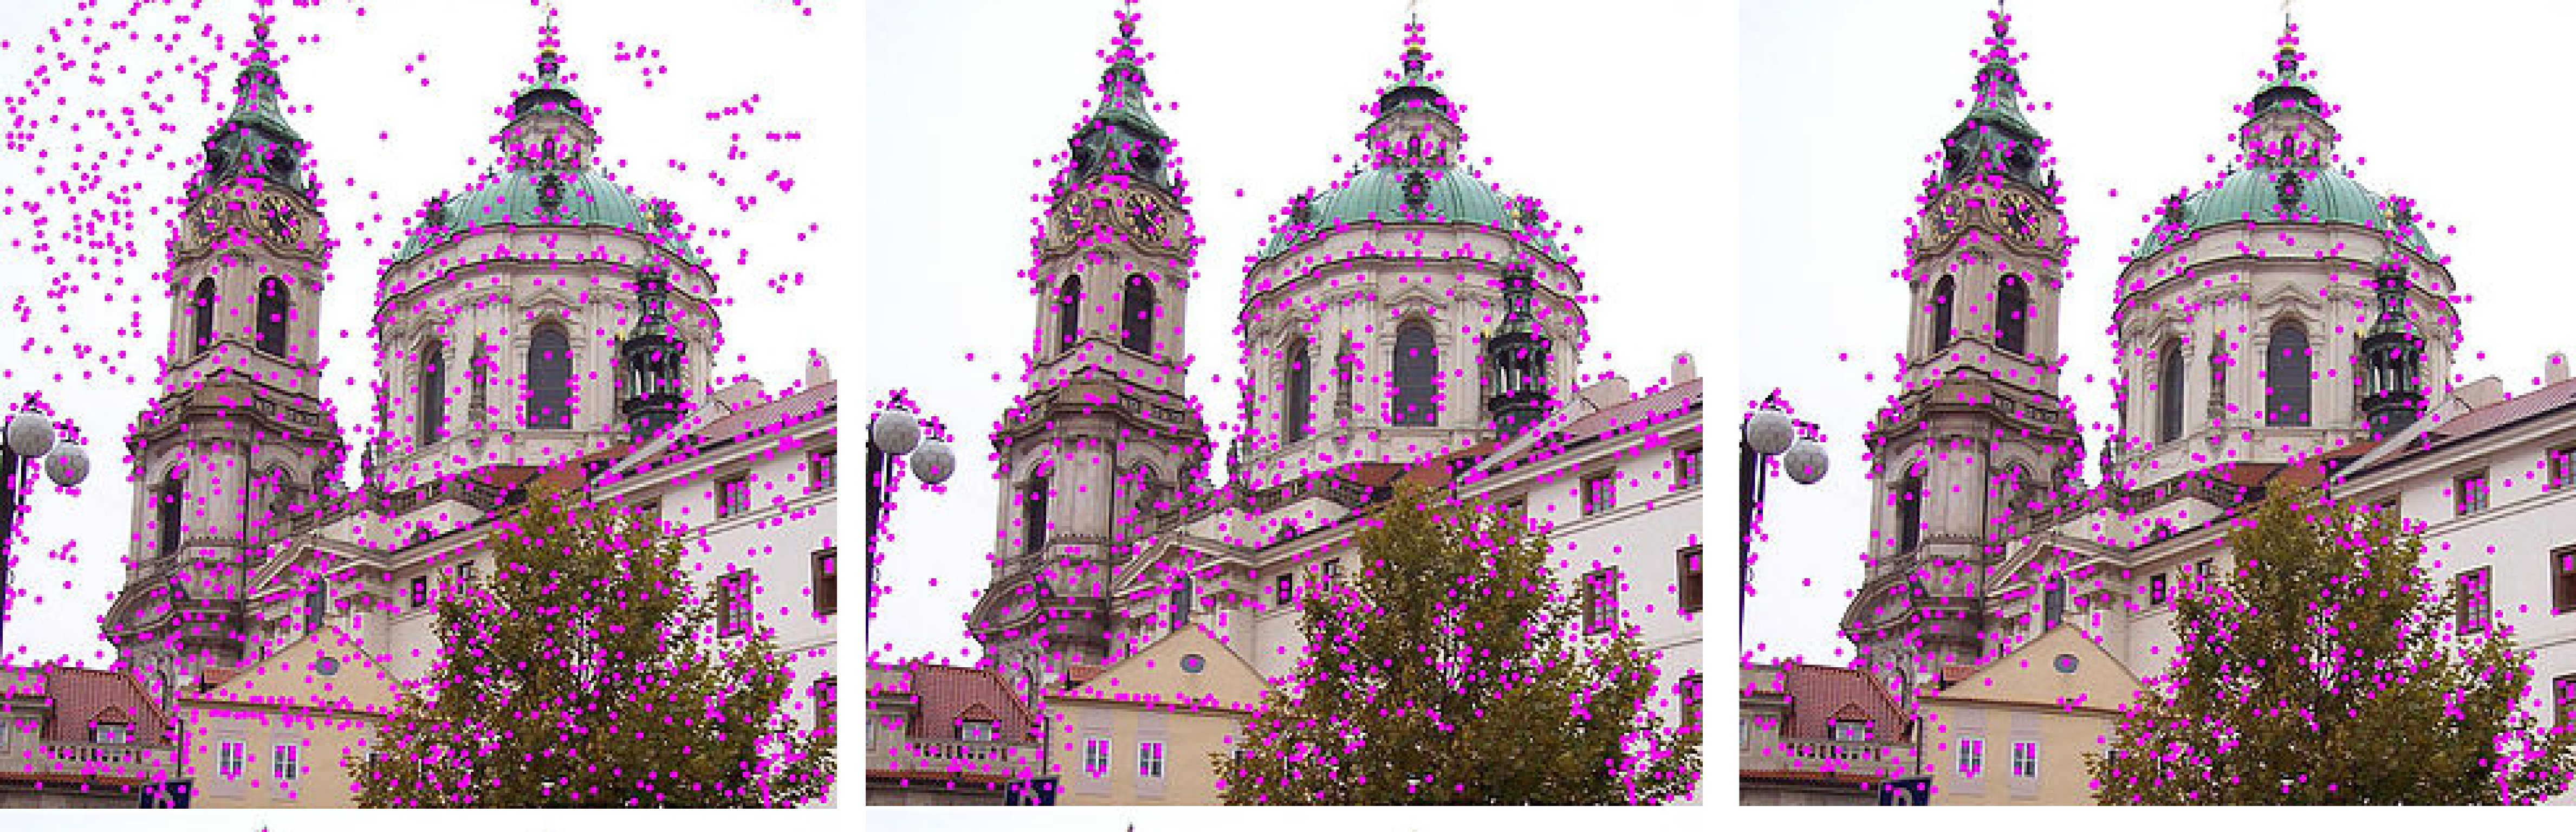
\includegraphics[width=\textwidth]{figs/siftrejection.png}
	% \caption{After scale space extrema are detected (left), the SIFT algorithm discards low contrast keypoints (center) and then filters out those located on edges (right). \copyright Lukas Mach CC-BY 3.0}
	\caption{在检测到尺度空间极值后(左),SIFT算法丢弃对比度低的关键点(中),然后过滤掉位于边缘的那些点(右)。 \copyright Lukas Mach CC-BY 3.0}
	\label{fig:siftrejection}
\end{figure}

% \item Reject extrema that are along edges by looking at the second derivative around each extrema (Figure \ref{fig:siftrejection}, right). Edges have a much larger principal curvature across them than along them.
% \item Assign a ``magnitude'' and ``orientation'' to each remaining extrema (keypoint). The magnitude is the squared difference between neighboring pixels and the orientation is the angle between magnitude along the y-axis vs. magnitude along the x-axis. These calculations are made for all pixels in a fixed neighborhood around the initial keypoint, e.g., in a 16x16 pixel neighborhood.
% \item Collect orientations of neighboring pixels in a histogram, e.g., 36 bins each covering 10 degrees. Maintain the orientation corresponding to the strongest peak and associate it with the keypoint.
% \item Repeat step 4, but for four 4x4 pixel areas around the keypoint in the image scale that has the most extreme minima/maxima. Here, only 8 bins are used for the orientation histogram. As there are 16 histograms in a 16x16 pixel area, the feature descriptor has 128 dimensions.
% \item The feature descriptor vector is normalized, tresholded, and again normalized to make it more robust against illumination changes.
% \item Local gradient magnitude and orientation are grouped into bins and create a 128-dimensional feature descriptor.

\item 通过查看每个极值处二阶导数来排除边缘的极值(图\ref{fig:siftrejection},右)。穿过边缘的主曲率比沿着它们的大得多。
\item 为每个剩余的极值(关键点)分配一个“大小”和“方向”。大小是相邻像素之间的平方差,方向是沿着$y$轴的幅度与沿$x$轴的幅度之间的角度。这些计算是针对初始关键点周围的固定邻域中的所有像素进行的,例如在$16\times 16$像素邻域中。
\item 收集直方图中相邻像素的方向,例如组数为36,组距为10度。保留与最强峰对应的方向,并将其与关键点相关联。
\item 只对图像尺度中关键点周围的有最小值/最大值的的四个$4\times 4$像素区域,重复步骤4。在这里,方向直方图组数为8。由于$16\times 16$像素区域中有16个直方图,所以特征描述符有128维。
\item 特征描述符向量被归一化、阈值化,并再次归一化,使其对明暗变化更加鲁棒。
\item 局部梯度大小和方向被分组成仓并创建128维特征描述符。

\end{enumerate}

% The resulting 128 dimensional feature vectors are now scale-invariant (due to step 2), rotation-invariant (due to step 5), and robust to illumination changes (due to step 7).

所得到的128维特征向量现在是尺度不变的(由于步骤2)、旋转不变的(由于步骤5),并且对明暗变化(由于步骤7)是鲁棒的。

% \subsection{Object Recognition using scale-invariant features}
% Scale-invariant features of training images can be stored in a database and can be used to identify these objects in the future. This is done by finding all features in an image and comparing them with those in the database. This comparison is done by using the Euclidian distance as metric and searching a k-d tree (with d=128). In order to make this approach robust, each object needs to be identified by at least 3 independent features. For this, each descriptor stores the location, scale and orientation of it relative to some common point on the object. This allows each detected feature to ``vote'' for the position of the object that it is most closely associated with in the database.  This is done using a Hough-transform. For example, position (2 dimensions) and orientation (1 dimension) can be discretized into bins (30 degree width for orientation); bright spots in Hough-space then correspond to an object pose that has been identified by multiple features.

\subsection{使用比例不变特征的对象识别}

训练图像的尺度不变特征可以存储在数据库中,并可用于在将来识别这些对象。这是通过查找图像中的所有特征并将其与数据库中的特征进行比较来完成的。该比较通过使用欧几里得距离作为度量并搜索k-d树(d=128)来完成。为了使这一方法变得稳健,每个对象需要通过至少3个独立的特征来识别。为此,每个描述符存储相对于对象上某些公共点的位置、尺度和方向。这使每个检测到的特征对于与数据库中最密切相关联的对象的位置进行“投票”。这利用了霍夫变换。例如,位置(2维)和方向(1维)可以离散成组(方向以30度为宽度);然后霍夫空间中的亮点对应于已被多个特征识别的物体姿态。

% \section*{Take-home lessons}
\section*{课后补充}
\begin{enumerate}
% \item Features are ``interesting'' information in sensor data that are robust to variations in rotation and scale as well as noise.
% \item Which features are most useful depends on the characteristics of the sensor generating the data, the structure of the environment, and the actual application.
% \item There are many feature detectors available some of which operating as simple filters, others relying on machine learning techniques.
% \item Lines are among the most important features in mobile robotics as they are easy to extract from many different sensors and provide strong clues for localization.

\item 特征是传感器数据中的“有趣”信息,对于旋转和尺度以及噪声的变化都是鲁棒或稳健的。
\item 哪些特征最有用取决于生成数据的传感器的特性、环境结构和实际应用。
\item 有许多特征检测器可用,其中一些作为简单的过滤器,其他一些特征检测器依靠机器学习技术。
\item 直线是移动机器人中最重要的特征之一,因为它们易于从许多不同的传感器中提取,并为定位提供强大的线索。
\end{enumerate}

% \section*{Exercises}\small
\section*{习题}\small
\begin{enumerate}
% \item Think about what information would make good features in different operating scenarios: a supermarket, a warehouse, a cave.
% \item What other features could you detect using a Hough transform? Can you find parameterizations for a circle, a square or a triangle?
% \item Do an online search for SIFT. What other similar feature detectors can you find? Which provide source code that you can use online?
% \item A line can be represented by the function $y=mx+c$. Then, the Hough-space is given by a 2D coordinate system spanned by $m$ and $c$.

\item 思考什么信息会在不同的操作场景下产生好的特征:超市、仓库、洞穴。
\item 你可以使用霍夫变换检测哪些其他特征?你能找到一个圆、一个正方形或三角形的参数化吗?
\item 上网查询SIFT。你能找到什么其他类似的特征检测器?哪些提供可以开源使用的源代码?
\item 一条直线可以由函数$y=mx+c$表示。然后,霍夫空间由一个由$m$和$c$定义的二维坐标系给出。
\begin{enumerate}
% \item Think about a line representation in polar coordinates. What components has the Hough-space in this case?
% \item Derive a parameterization for a circle and describe the resulting Hough space.

\item 想想极坐标中的直线表示。在这种情况下哪些部分有霍夫空间?
\item 推导出圆的参数化,并描述生成的霍夫空间。
\end{enumerate}
\end{enumerate}
\normalsize

